\documentclass[11pt,a4paper]{article}

\usepackage[margin=2.5cm]{geometry}
\usepackage[T1]{fontenc}
\usepackage[utf8]{inputenc}
\usepackage{array}
\usepackage{booktabs}
\usepackage{longtable}
\usepackage{hyperref}
\usepackage{xcolor}
\usepackage{listings}
\usepackage{tikz}
\usepackage{amssymb}
\usetikzlibrary{positioning,arrows.meta}

\hypersetup{
  colorlinks=true,
  linkcolor=blue,
  urlcolor=blue
}

\newcommand{\artifact}[1]{\texttt{#1}}

\lstset{
  basicstyle=\ttfamily\small,
  breaklines=true,
  frame=single,
  columns=fullflexible,
  keepspaces=true,
  showstringspaces=false
}

\title{Plant Management Ontology Project Report}
\author{Ambrus Toth (), Florian Krieger (11924605), Viktor Hoffmann ()}

\date{\today}

\begin{document}

\maketitle

\section*{LLM Use Disclaimer}

An LLM was used during this exercise to support drafting, code cleanup, and
debugging. The submitted ontology, mappings, scripts, queries, and report text
were reviewed, adapted, and verified by the author.

% -----------------------------------------------------------------------
% Sections: Introduction + Domain and Application Idea
% Paste into your main report document as needed.
% -----------------------------------------------------------------------

\section{Introduction}

This report documents the design and implementation of a knowledge-graph-based
plant management system developed as part of the SAIKS assignment.
The system covers five steps: ontology engineering, knowledge graph creation
through OBDA, verification of semantic structures, ontology alignment, and a
RAG application.

The data foundation is the Trefle open plant dataset, which provides scientific
and common names, taxonomy, morphological attributes, geographic distributions,
and growth properties for over 400\,000 plant species.
A small generated shop inventory extends the dataset with retail-relevant
attributes such as stock, price, care level, and temperature preference.
All steps build on a shared OWL\,2 ontology and a GraphDB knowledge graph
materialized from a normalized SQLite database.

\section{Domain and Application Idea}

\subsection{Problem Domain}


The domain is plant management for a small specialist plant shop, considered
from two perspectives.
\begin{itemize}
    \item \textbf{Shop perspective.}
Staff need to manage inventory and answer product questions: which species are
stocked, at what price, in what quantity, how long they have been on the shelf,
and what care level they require.
\item \textbf{Customer perspective.}
Customers need to find plants that match personal criteria: growth habit,
flower or foliage colour, edibility, climate suitability, or ease of care.
\end{itemize}

A single knowledge graph spanning botanical facts and retail state lets both
needs be served from one source, for example finding low-maintenance edible
plants from tropical regions that are currently in stock.

\subsection{Application Idea}

The target application is a natural-language query interface over the
plant knowledge graph.
A shop employee or customer types a question in plain English.
The system retrieves relevant ontology terms and named entities from the graph,
sends them together with the question to a language model, and executes the
generated SPARQL query against a local GraphDB instance.
The language model then produces a short factual answer grounded in the query
result.

The application is deliberately read-only and shop-scoped: it is not a general
botanical database but a decision-support tool for a shop context, where
questions about stock, care, and plant properties need to be answered quickly
without expert knowledge of SPARQL or taxonomy.

\subsection{Competency Questions}

The ontology and knowledge graph were designed to answer the following
representative competency questions.

\begin{enumerate}
  \item Which plants belong to a given family or genus?
  \item Which plants bloom in a given month or season?
  \item Which plants have edible parts, and what parts are they?
  \item Which plants are suitable for a given growth habit
        (e.g.\ tree, shrub, annual)?
  \item Which shop products are currently low in stock?
  \item Which shop products are easy-care warm-temperature plants?
  \item Which plants have been in the shop inventory for a long time?
  \item Which plants have a specific flower, fruit, or foliage colour?
  \item Which plants are distributed in a given geographic region?
  \item Which edible plants from a specific family are available in the shop?
\end{enumerate}

These questions guided the class hierarchy, property selection, and named
individual design of the ontology and determined which attributes were
included in the R2RML mapping and materialized into the knowledge graph.


\section{Step 1: Ontology Engineering}

The base ontology is generated by \artifact{scripts/generate\_ontology.py} and
stored as \artifact{ontology/ plant\_management.ttl}.
After an OOPS scan and targeted fixes, the submission artifact is
\artifact{ontology/plant\_management\_oops\_fixed.ttl}, which contains
1\,127 triples, 37 classes, 48 object properties, 33 datatype properties,
and 86 named individuals.

\subsection{Modelling Choices}

The central class is \texttt{Plant}, representing one species.
Taxonomy is modelled as a class hierarchy (\texttt{Family}, \texttt{Genus})
linked by object properties and a \texttt{propertyChainAxiom} so that the
family of a plant can be inferred transitively through its genus.
Controlled vocabularies such as growth habit, care level, season, and
temperature preference are modelled as named individuals of dedicated classes
rather than plain string literals, enabling SPARQL filtering and class-level
reasoning.
Temporal values such as bloom, fruit, and growth months are represented as
object properties pointing to twelve named \texttt{Month} individuals,
which supports month- and season-range queries.
The shop extension adds a \texttt{ShopProduct} class linked to \texttt{Plant}
with datatype properties for price, stock, and days on shelf.

\subsection{OWL\,2 Features}

The ontology uses OWL\,2 features beyond the OWL\,1 baseline to improve
expressivity and support reasoning:

\begin{itemize}
  \item \texttt{AllDisjointClasses} and \texttt{disjointUnionOf} for
        controlled vocabularies such as \texttt{GrowthHabit} and
        \texttt{Season}, preventing invalid class combinations.
        In description logic this reads:
        \[
          \texttt{GrowthHabit} \equiv \texttt{Tree} \sqcup \texttt{Shrub}
          \sqcup \texttt{Annual} \sqcup \cdots, \qquad
          \texttt{Tree} \sqcap \texttt{Shrub} \sqsubseteq \bot
        \]
  \item \texttt{propertyChainAxiom} to infer plant-to-family membership
        through genus:
        \[
          \texttt{hasGenus} \circ \texttt{hasFamily} \sqsubseteq \texttt{hasFamily}
        \]
  \item \texttt{TransitiveProperty} on \texttt{hasAncestorTaxon} for
        hierarchical taxonomy traversal;
  \item \texttt{FunctionalProperty} on single-valued attributes such as
        \texttt{hasTrefleId} and \texttt{hasScientificName};
  \item \texttt{someValuesFrom} and \texttt{allValuesFrom} existential and
        universal restrictions, e.g.\
        $\texttt{Plant} \sqsubseteq \exists\,\texttt{hasPart.PlantPart}$
        and
        $\texttt{PlantDistribution} \sqsubseteq \forall\,\texttt{inRegion.Region}$;
  \item \texttt{minQualifiedCardinality} to require at least one
        \texttt{PlantDistribution} node per distributed plant;
  \item \texttt{hasKey} to declare \texttt{hasTrefleId} as a unique key for
        \texttt{Plant} individuals;
  \item XSD datatype ranges (\texttt{xsd:integer}, \texttt{xsd:decimal},
        \texttt{xsd:date}) on all numeric and date properties.
\end{itemize}

\subsection{Ontology Design Patterns}

Three established ontology design patterns (ODPs) are used to handle
structurally complex parts of the domain.
\begin{itemize}
    \item \textbf{Componency.}
Plant parts (flower, fruit, foliage, root) are modelled as component classes
linked to \texttt{Plant} via \texttt{hasPart} and \texttt{isPartOf}.
This separates part-level attributes such as colour and texture from the plant
itself and allows queries over individual parts without reifying the whole plant.

\begin{center}
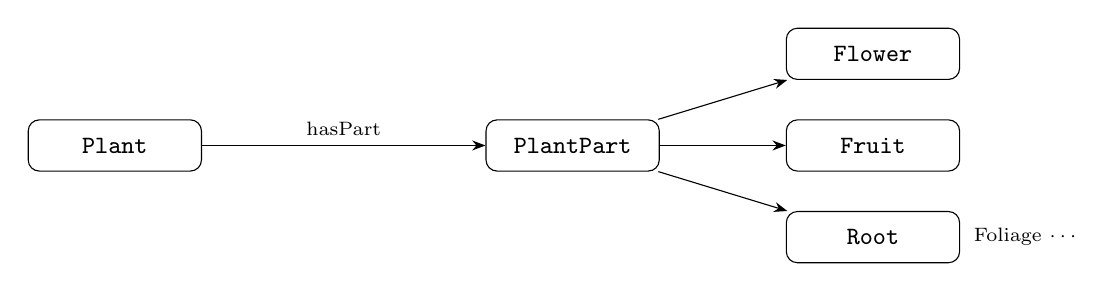
\begin{tikzpicture}[
  node/.style={draw, rounded corners, minimum width=2.2cm,
               minimum height=0.65cm, font=\small\ttfamily},
  >=Stealth
]
  \node[node] (plant) {Plant};
  \node[node, right=3.6cm of plant] (part) {PlantPart};
  \node[node, above right=0.5cm and 1.6cm of part] (flower) {Flower};
  \node[node, right=1.6cm of part]                 (fruit)  {Fruit};
  \node[node, below right=0.5cm and 1.6cm of part] (root)   {Root};

  \draw[->] (plant) -- node[above, font=\scriptsize] {hasPart} (part);
  \draw[->] (part)  -- (flower);
  \draw[->] (part)  -- (fruit);
  \draw[->] (part)  -- (root);
  \node[font=\scriptsize, right=0.05cm of root] {Foliage $\cdots$};
\end{tikzpicture}
\end{center}

\item \textbf{N-ary Relation.}
Geographic distribution cannot be expressed as a binary property because each
distribution record carries both a region and a presence status
(native, introduced, etc.).
A reified \texttt{PlantDistribution} node connects \texttt{Plant},
\texttt{Region}, and \texttt{PresenceStatus}, following the W3C N-ary
relation pattern.

\begin{center}
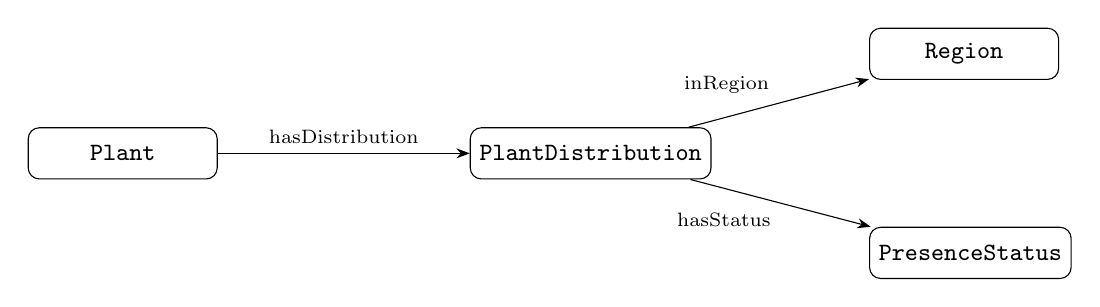
\begin{tikzpicture}[
  node/.style={draw, rounded corners, minimum width=2.4cm,
               minimum height=0.65cm, font=\small\ttfamily},
  >=Stealth
]
  \node[node] (plant) {Plant};
  \node[node, right=3.2cm of plant] (dist) {PlantDistribution};
  \node[node, above right=0.6cm and 2.0cm of dist] (region) {Region};
  \node[node, below right=0.6cm and 2.0cm of dist] (status) {PresenceStatus};

  \draw[->] (plant)  -- node[above, font=\scriptsize] {hasDistribution} (dist);
  \draw[->] (dist)   -- node[above left, font=\scriptsize] {inRegion} (region);
  \draw[->] (dist)   -- node[below left, font=\scriptsize] {hasStatus} (status);
\end{tikzpicture}
\end{center}

\item \textbf{AgentRole.}
Plant uses (edible, medicinal, ornamental, vegetable) are modelled as roles
rather than flat string values.
A plant can simultaneously be edible and ornamental, or medicinal and a
vegetable - categories that overlap in practice but must remain
distinguishable for queries such as \emph{``which edible plants are not
vegetables?''}.
A \texttt{PlantUse} class with subclasses for each use type allows a plant to
carry multiple non-exclusive roles and supports role-based filtering in SPARQL.


\end{itemize}






\section{Step 2: KG Creation Through OBDA}

The knowledge graph is created from a relational SQLite database that combines
the Trefle species dump with a generated shop inventory. Trefle provides the
botanical data, while the shop inventory adds product-level information such as
stock, price, care level, and shelf date. Together, these sources cover both
plant-centred and shop-centred competency questions.

\subsection{Data Preparation}

The Trefle file is a tab-separated species dataset with taxonomy, names,
morphology, ecology, cultivation values, distribution strings, images, and
external links. The shop inventory is generated from selected genera and
families that are typical for a small plant shop, for example Araceae,
Orchidaceae, Lamiaceae, Cactaceae, Geraniaceae, and Rosaceae.

The generated shop file contains 95 product rows. Each row stores a product id,
the Trefle id used as foreign key, a shop product name, stock quantity, price in
euro, shelf date, care level, and temperature category. Care level is either
overridden for common shop products or derived from Trefle ecological values.
The shop data is generated in a way so that the competency questions can be
asked. For example, some products are older than 90 days.

\subsection{Relational Schema}

The loader normalises the CSV fields into separate relational tables. Single
valued attributes, such as scientific name, pH values, height values, and
Wikipedia URL, are stored in \artifact{plant}. Taxonomy is separated into
\artifact{family} and \artifact{genus}. Multi-value CSV fields are stored in
link tables, for example \artifact{plant\_common\_name},
\artifact{plant\_synonym}, \artifact{plant\_growth\_habit},
\artifact{plant\_bloom\_month}, \artifact{plant\_edible\_part}, and
\artifact{plant\_distribution}. Plant parts are stored as component tables for
flowers, foliage, and fruits. Controlled shop values are stored as small
dimension tables for care level and temperature category.

This structure keeps the R2RML mapping direct: most triples maps read one table
or one simple join, and repeated values are not encoded as comma-separated
strings in the relational database.

\begin{table}[h]
\centering
\begin{tabular}{lr}
\toprule
Table & Rows \\
\midrule
\artifact{plant} & 416,473 \\
\artifact{family} & 580 \\
\artifact{genus} & 15,540 \\
\artifact{plant\_common\_name} & 75,198 \\
\artifact{plant\_synonym} & 633,831 \\
\artifact{plant\_growth\_habit} & 33,903 \\
\artifact{plant\_bloom\_month} & 6,668 \\
\artifact{flower\_component} & 5,984 \\
\artifact{foliage\_component} & 3,250 \\
\artifact{fruit\_component} & 2,565 \\
\artifact{region} & 368 \\
\artifact{plant\_distribution} & 1,306,113 \\
\artifact{shop\_product} & 95 \\
\bottomrule
\end{tabular}
\caption{Selected SQLite table sizes in \artifact{data/plantms.db}.}
\label{tab:sqlite-table-sizes}
\end{table}

All 95 shop products join successfully to a plant row through the Trefle id. The
current shop inventory contains 634 units in stock. The average product price is
17.08 euro, with prices ranging from 3.00 euro to 70.60 euro. The generated
inventory contains 62 easy-care product lines and 33 medium-care product lines;
no hard-care product line is present in the current generated file. By
temperature category, the inventory contains 26 cool, 34 moderate, and 35 warm
product lines.

\subsection{R2RML Mapping}

The mapping file is \artifact{plant\_management\_r2rml.ttl}. It contains
32 triples maps and 71 predicate-object maps. The mappings create IRIs in the
\artifact{http://www.semanticweb.org/plantms/resource/} namespace, for example
\artifact{/plant/\{plant\_id\}}, \artifact{/family/\{family\_name\}},
\artifact{/genus/\{genus\_name\}}, \artifact{/distribution/\{plant\_id\}/\{region\_id\}},
and \artifact{/product/\{product\_id\}}.

The main plant triples map assigns \artifact{plant:Plant} and maps labels,
Trefle identifiers, scientific names, publication metadata, image and Wikipedia
links, ecological numeric values, pH values, height values, and boolean edible
or vegetable flags. Parent triples maps link plants to family and genus
individuals. Other mappings cover common names, synonyms, growth descriptors,
month links, edible parts and plant uses, component nodes for flowers, foliage,
and fruits, colour values, distribution nodes, regions, and shop products.

\begin{figure}[h]
\centering
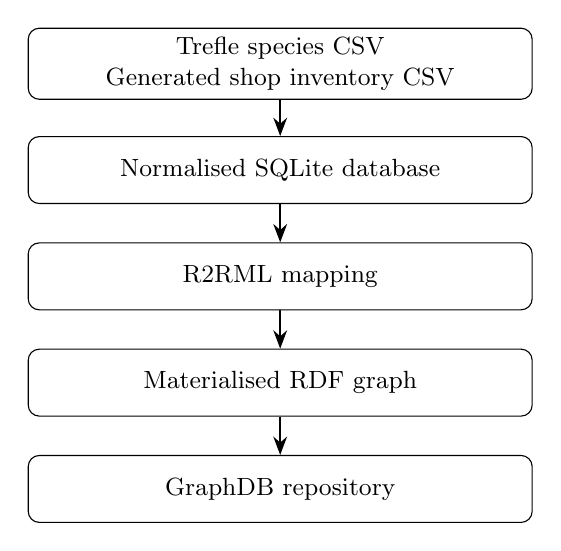
\begin{tikzpicture}[
  flowstep/.style={
    draw,
    rounded corners,
    align=center,
    minimum width=6.4cm,
    minimum height=0.85cm,
    font=\small
  },
  arrow/.style={->, thick, >=Stealth}
]
  \node[flowstep] (csv) at (0,0) {\shortstack{Trefle species CSV\\Generated shop inventory CSV}};
  \node[flowstep] (sqlite) at (0,-1.35) {Normalised SQLite database};
  \node[flowstep] (r2rml) at (0,-2.70) {R2RML mapping};
  \node[flowstep] (rdf) at (0,-4.05) {Materialised RDF graph};
  \node[flowstep] (graphdb) at (0,-5.40) {GraphDB repository};

  \draw[arrow] (csv) -- (sqlite);
  \draw[arrow] (sqlite) -- (r2rml);
  \draw[arrow] (r2rml) -- (rdf);
  \draw[arrow] (rdf) -- (graphdb);
\end{tikzpicture}
\caption{Pipeline from Trefle and shop CSV files through SQLite and R2RML mappings to the materialised knowledge graph.}
\label{fig:obda-pipeline}
\end{figure}

\subsection{Materialisation and GraphDB Import}

Ontop CLI 5.4.0 was tested locally with the SQLite database and the R2RML
mapping. In the tested environment, Ontop generated SQLite SQL that failed near
\artifact{UNION} for predicates produced by several triples maps. Therefore, the
full ABox was materialised with the project materialisation script. This follows
the same relational schema and predicate structure as the R2RML mapping, but
writes the triples directly.

The materialisation resulted in \artifact{data/plantms\_full\_kg.ttl}. The
current materialisation log reports 11,111,501 triples and a runtime of
80.0 seconds. The result contains 416,473 \artifact{plant:Plant} instances,
580 family resources, 15,540 genus resources, 1,306,113 plant-distribution rows
represented as reified \artifact{plant:PlantDistribution} nodes, and
95 \artifact{plant:ShopProduct} instances.

The GraphDB repository uses the default GraphDB 10.8 inference ruleset
\artifact{rdfsplus-optimized}. This ruleset was chosen because it provides RDFS
reasoning together with selected OWL features, including inverse and transitive
properties. This is sufficient for the ontology features used in the project
without switching to a broader and more expensive OWL ruleset. After importing
the materialised KG and the OOPS-fixed ontology, GraphDB reported 11,105,948
explicit statements, 6,977,509 inferred statements, and 18,083,457 total
statements.

\section{Step 3: Verification of Semantic Structures}

Step 3 has two parts. The ontology was checked with the OOPS! pitfall scanner
and then corrected with a reproducible follow-up script. The materialised KG was
checked with SHACL rules stored in Turtle format. This follows the assignment
requirement to document both ontology verification and KG verification.

\subsection{OOPS Scan}

The OOPS scan reported five categories of issues. They were not all modelling
errors, but they were useful for reviewing the ontology and improving the final
result.

\begin{table}[h]
\centering
\begin{tabular}{lllr}
\toprule
Pitfall & Severity & Meaning & Count \\
\midrule
P19 & Critical & Multiple domains or ranges & 16 \\
P29 & Critical & Wrong transitive relationships & 2 \\
P41 & Important & Missing licence & 1 \\
P04 & Minor & Unconnected ontology elements & 3 \\
P13 & Minor & Missing inverse relationships & 19 \\
\bottomrule
\end{tabular}
\caption{OOPS findings from the first scan, ordered by severity.}
\label{tab:oops-findings}
\end{table}

\begin{table}[h]
\centering
\begin{tabular}{p{0.12\linewidth}p{0.36\linewidth}p{0.42\linewidth}}
\toprule
Pitfall & Project example & Possible effect in the KG \\
\midrule
P19 &
\artifact{product/1001} is a Monstera product with
\artifact{hasPriceEur} 32.61 and \artifact{hasStockQuantity} 5. &
If numeric ranges are modelled ambiguously, valid shop values such as prices
and stock counts could be interpreted under an unintended combined datatype
range. \\
P29 &
\artifact{plant/101119} represents \emph{Abies balsamea}; it has a generated
flower component with yellow flower colour. &
If \artifact{hasPart} remains transitive, indirect component relations could be
returned as if they were direct plant parts, making part-level queries less
precise. \\
P04 &
\artifact{Abutilon theophrasti} blooms in June and July, but an unconnected
\artifact{Season} class would not connect those month values to summer. &
Month-to-season questions would not be supported by the ontology structure. \\
P13 &
\artifact{Monstera obliqua} belongs to family \artifact{Araceae}; product
\artifact{1004} is a \artifact{Peace Lily} with care level \artifact{Easy}. &
Without inverse properties, reverse questions such as ``which plants are in
Araceae?'' or ``which products are easy-care?'' require less direct query
patterns. \\
P41 &
The ontology header did not declare a licence. &
This does not change instance reasoning, but it makes the submission result less
clear for reuse and publication. \\
\bottomrule
\end{tabular}
\caption{Concrete project examples for the first OOPS findings.}
\label{tab:oops-instance-examples}
\end{table}

P19 needed attention because multiple range declarations in OWL are interpreted
as an intersection, not as alternatives. In this ontology, this affected numeric
properties such as \artifact{hasPriceEur}, \artifact{hasStockQuantity},
\artifact{hasLightRequirement}, and \artifact{hasPhMinimum}. If left unclear,
validators and reasoners could treat valid product prices, stock quantities, or
Trefle scale values as belonging to an unintended combined datatype range.

P29 was also critical because transitive part relations can lead to unwanted
inferences if the domain and range are too narrow. For example, if
\artifact{hasPart} were transitive, a plant with a flower and a flower with a
smaller part could make all intermediate resources behave like direct plant
parts in queries. This would make component-level queries less reliable.

P41 did not affect reasoning, but the missing licence was still important for a
submission result. P04 showed that \artifact{Season},
\artifact{TaxonomicRank}, and \artifact{TimeInterval} needed to be reviewed.
For example, an unconnected \artifact{Season} class would not support the
intended month-to-season questions. P13 was minor, but missing inverse
properties would make reverse navigation harder, such as asking which plants
belong to a family or which products use a certain care level.

\subsection{OOPS Fixes}

The OOPS fixes are reproducible with
\artifact{scripts/apply\_oops\_fixes.py}. This script reads the original ontology
file and writes separate fixed files:
\artifact{ontology/plant\_management\_oops\_fixed.ttl} and
\artifact{ontology/plant\_management\_oops\_fixed.rdf}.

\begin{table}[h]
\centering
\begin{tabular}{lr}
\toprule
Metric & Count \\
\midrule
Triples & 1,127 \\
Classes & 37 \\
Object properties & 48 \\
Datatype properties & 33 \\
Named individuals & 86 \\
\bottomrule
\end{tabular}
\caption{OOPS-fixed ontology metrics.}
\label{tab:oops-fixed-metrics}
\end{table}

The fixes remove the unused \artifact{TimeInterval} class and connect
\artifact{Season} to \artifact{Month} through \artifact{inSeason} and
\artifact{hasMonth}. The abstract \artifact{TaxonomicRank} class is kept because
it is still used as the superclass of \artifact{Family} and \artifact{Genus}.
Useful inverse properties are added for taxonomy, months, regions, plant uses,
edible parts, care levels, temperature categories, growth descriptors, colours,
and conditions. The script removes transitivity from \artifact{hasPart} and
\artifact{isPartOf}, removes the part propagation property chain, rewrites the
restricted numeric datatype ranges so that each affected property has one range
declaration, and adds a CC BY 4.0 licence.

The implemented changes result in the OOPS-fixed ontology file used in the
later KG, SHACL, and RAG steps. A second OOPS scan of the fixed ontology shows
only minor findings. No critical or important issue remains in the scan result.

\begin{table}[h]
\centering
\begin{tabular}{lllr}
\toprule
Pitfall & Severity & Meaning & Count \\
\midrule
P04 & Minor & Unconnected ontology elements & 1 \\
P20 & Minor & Misusing ontology annotations & 5 \\
\bottomrule
\end{tabular}
\caption{OOPS findings from the second scan after applying the fixes.}
\label{tab:oops-second-scan}
\end{table}

The remaining P04 warning concerns \artifact{TaxonomicRank}. This class is kept
as an abstract superclass for \artifact{Family} and \artifact{Genus}. The P20
warnings concern annotation properties on inverse helper properties, for example
\artifact{isFruitingMonthOf}, \artifact{temperatureCategoryOfProduct},
\artifact{isGrowthMonthOf}, \artifact{careLevelOfProduct}, and
\artifact{isBloomMonthOf}. These warnings affect documentation quality rather
than ontology consistency or KG reasoning.

\subsection{SHACL Validation}

The SHACL rules are stored in
\artifact{plant\_management\_shapes.ttl}. The file contains 12 node shapes,
37 property constraints, and 2 SPARQL constraints. This is more than the
required 5--10 SHACL rules, but the checks remain grouped by domain area and
are still easy to inspect.

\begin{table}[h]
\centering
\begin{tabular}{ll}
\toprule
Rule area & Main checks \\
\midrule
Plant identity & Trefle id and scientific name \\
Taxonomy & optional genus/family links and required genus-family links \\
Numeric values & scale values, pH, height, price, and stock bounds \\
Temporal values & month links and season links \\
Plant parts & component links, colours, and foliage texture \\
Distribution & plant, region, and distribution status \\
Shop products & product id, name, plant link, care, and temperature \\
Cross checks & pH min/max and shop inverse link \\
\bottomrule
\end{tabular}
\caption{SHACL rule groups added for KG validation.}
\label{tab:shacl-rule-groups}
\end{table}

The identity and shop-product shapes use cardinality checks to ensure that
generated resources have required identifiers and labels. Numeric shapes check
Trefle scale values, pH values, measurements, prices, and stock quantities.
Object-property shapes check that linked resources belong to the expected
classes, for example \artifact{plant:Month}, \artifact{plant:Region}, and
\artifact{plant:CareLevel}. The SPARQL constraints check that minimum pH is not
greater than maximum pH and that plant-to-shop-product links are consistent in
both directions.

The validation report is stored in
\artifact{plant\_management\_validation\_report.ttl}. The selected course-tool
route is the TopBraid SHACL engine. The data graph consists of the materialised
KG and \artifact{ontology/plant\_management\_oops\_fixed.ttl}; the shapes graph
is \artifact{plant\_management\_shapes.ttl}. The exported report contains no
validation result entries and states that the graph conforms:

\begin{lstlisting}[caption={SHACL validation result in plant\_management\_validation\_report.ttl.}]
sh:conforms true
\end{lstlisting}

\section{Step 4: Ontology Alignment}

The assignment asks for an alignment between the project ontology and another
ontology from the same domain, with a short discussion of strengths and
weaknesses. The available alignment result is
\artifact{plant\_management\_po\_alignment.ttl}. It aligns the local ontology
with the Plant Ontology (PO), which uses the namespace
\artifact{http://purl.obolibrary.org/obo/}. The file imports
\artifact{http://purl.obolibrary.org/obo/po.owl}.
% TODO: add tool-generated Alignment API file if required for final submission.

\subsection{Choice of External Ontology}

PO was selected because it directly describes plant structures such as flowers,
fruits, roots, and leaves. This makes it a better fit for the local plant-part
model than broader agriculture or environment vocabularies.

\begin{table}[h]
\centering
\begin{tabular}{lll}
\toprule
Candidate & Fit & Reason \\
\midrule
Plant Ontology & Best & Direct match for plant structures \\
Plant Trait Ontology & Good & Useful for traits, but less direct for classes \\
AGROVOC & Medium & Broad agriculture thesaurus \\
Crop Ontology & Medium-low & More focused on crop breeding variables \\
ENVO & Medium-low & Useful for environment, not plant parts \\
NCBI Taxonomy & Low & Needs taxon ids that are not in the data \\
\bottomrule
\end{tabular}
\caption{Checked ontology candidates for Task 4.}
\label{tab:alignment-candidates}
\end{table}

\subsection{Alignment Result}

The current alignment is manual and conservative. It contains three
\artifact{owl:equivalentClass} mappings with matching
\artifact{skos:exactMatch} statements, one \artifact{rdfs:subClassOf} mapping
from the local generic plant-part class to the PO plant-structure class, and two
\artifact{skos:closeMatch} statements.

\begin{table}[h]
\centering
\begin{tabular}{lll}
\toprule
Local concept & PO concept & Relation \\
\midrule
\artifact{plant:PlantPart} & \artifact{po:PO\_0009011} & subclass and close match \\
\artifact{plant:Flower} & \artifact{po:PO\_0009046} & equivalent class and exact match \\
\artifact{plant:Fruit} & \artifact{po:PO\_0009001} & equivalent class and exact match \\
\artifact{plant:Root} & \artifact{po:PO\_0009005} & equivalent class and exact match \\
\artifact{plant:Foliage} & \artifact{po:PO\_0025034} & close match \\
\bottomrule
\end{tabular}
\caption{Mappings in \artifact{plant\_management\_po\_alignment.ttl}.}
\label{tab:po-alignment}
\end{table}

Exact mappings are used only where the two ontologies describe the same
botanical structure. \artifact{plant:Flower}, \artifact{plant:Fruit}, and
\artifact{plant:Root} therefore use \artifact{owl:equivalentClass}. The local
\artifact{plant:PlantPart} class is broader as a modelling helper, so it is only
connected to the PO plant-structure class through a subclass relation and a
close match. \artifact{plant:Foliage} is aligned only as a close match to the PO
leaf concept because local foliage represents the visible leafy part of a shop
plant and is not exactly the same concept as the botanical PO leaf class.

\subsection{Strengths and Weaknesses}

The main strength of the alignment is that it is conservative. It avoids exact
matches for concepts that are only related, and it documents each mapping with a
short comment in the Turtle file. The mappings also focus on classes that are
actually used by the local ontology and generated data, so they are relevant for
the implemented project.

The main weakness is that the current result is not a tool-generated
Alignment API result file. It also covers only the plant-structure part of the
ontology. Other areas, such as taxonomy, ecological conditions, distribution,
plant uses, and shop inventory, are not aligned because PO does not model those
project-specific aspects in the same way. The alignment therefore improves
interoperability for plant anatomy, but it is not a complete cross-ontology
mapping for the whole plant-management domain.

\subsection{Comparison DBpedia}


The ontology was compared against DBpedia using automated SPARQL queries
and token Jaccard similarity matching. The full results are in
\artifact{data/dbpedia\_comparison\_report.md}.

\begin{itemize}
  \item \textbf{TBox coverage.}
    Of 253 retrieved DBpedia concepts, $\approx$160 are non-botanical
    (persons, athletes, animals) leaked in via DBpedia's general-purpose
    class hierarchy under \texttt{dbo:Species}.
    Filtering to plant-relevant concepts, our ontology covers $\approx$25--30\,\%,
    with exact matches for plant, genus, family, and scientific name.
    Gaps are finer taxonomy ranks (order, class, phylum) and conservation
    status, neither required for the shop domain.

  \item \textbf{Instance property coverage.}
    The four most common DBpedia properties across 30 sampled plants were
    \texttt{dbo:description}, \texttt{dbo:wikiPageWikiLink},
    \texttt{dbo:thumbnail}, and \texttt{dbo: wikiPageExternalLink} -
    all Wikipedia metadata, not botanical content.
    Our ontology correctly omits these; DBpedia's plant instances carry
    little structured botanical data beyond Wikipedia linking properties.

  \item \textbf{Structural depth.}
    Where both ontologies model the same concept, ours is more expressive:
    taxonomy uses a class hierarchy with a property chain rather than flat
    strings, and distribution uses a reified N-ary node instead of a single
    image URL. Plant parts are absent from DBpedia entirely.
    DBpedia covers conservation status, free-text abstracts, and
    geo-coordinates; our ontology adds bloom months, and
    edible parts as domain-specific extensions.
\end{itemize}


\section{Step 5: KG-Based RAG Application}

The RAG application answers natural-language plant questions from the GraphDB
knowledge graph using the SPARQL-generation route from lecture 4. This is
Approach \#1: the RDF graph remains in GraphDB and no vector index is created.

\subsection{Architecture}

The default pipeline has one retrieval path:

\begin{enumerate}
  \item \textbf{Ontology retrieval} -- the CLI searches ontology class and
    property labels for terms relevant to the natural-language question.
  \item \textbf{Entity linking} -- the CLI searches labeled KG entities for
    lexical matches, such as the family \artifact{Araceae}.
  \item \textbf{SPARQL generation} -- the configured LLM provider receives the
    question, retrieved schema terms, linked entities, and a few SPARQL
    examples. It returns a SPARQL \artifact{SELECT} query.
  \item \textbf{Query validation} -- the CLI rejects update operations and remote
    \artifact{SERVICE} calls and limits the maximum number of result rows.
  \item \textbf{SPARQL retrieval} -- the generated query is executed against the
    GraphDB SPARQL endpoint \artifact{http://localhost:7200/repositories/plantms}.
  \item \textbf{Grounded answer generation} -- the configured LLM receives only
    the question, executed query, and returned rows and produces a short factual
    answer.
\end{enumerate}

There is no vector index, embedding model, vector fallback, local KG mode, or
fixed-template mode. The CLI supports a local Ollama provider and an OpenAI Responses API provider.
For OpenAI, the API key is stored locally in an ignored \artifact{.env} file
loaded automatically by the CLI; the checked-in template is
\artifact{.env.example}. The
default OpenAI model is \artifact{gpt-5-mini}.

\subsection{Query Interface}

The CLI supports three modes:
\begin{enumerate}
\item \textbf{Interactive session}
\\python3 scripts/rag\_query.py

\item \textbf{Single query}
\\python3 scripts/rag\_query.py --query "What is the total stock of all Araceae plants in the shop?"

\item \textbf{Inspect retrieved terms and generated SPARQL}
\\python3 scripts/rag\_query.py --show-plan --query "What is the total stock of all Araceae plants in the shop?"

\item \textbf{Use OpenAI Responses API}
\\python3 scripts/rag\_query.py --provider openai --query "What is the total stock of all Araceae plants in the shop?"

\item \textbf{Run the dynamic GraphDB/SPARQL demo questions automatically}
\\python3 scripts/rag\_query.py --demo

\end{enumerate}

\section{Findings and Conclusion}


\end{document}
